\section{Character-based LSTM decoder for NMT}
\label{sec:char_dec}
We will now add a LSTM-based character-level decoder to our NMT system, based on Luong \& Manning's work.\footnote{Achieving Open Vocabulary Neural Machine Translation with Hybrid Word-Character Models, Luong and Manning, 2016. \url{https://arxiv.org/abs/1604.00788}}
The main idea is that when our word-level decoder produces an \texttt{<UNK>} token, we run our character-level decoder (which you can think of as a character-level conditional language model) to instead generate the target word one character at a time, as shown in Figure \ref{fig:char-decoder}. 
This will help us to produce rare and out-of-vocabulary target words.

\begin{figure}[h!]
    \begin{center}
        \captionsetup{width=0.8\textwidth}
        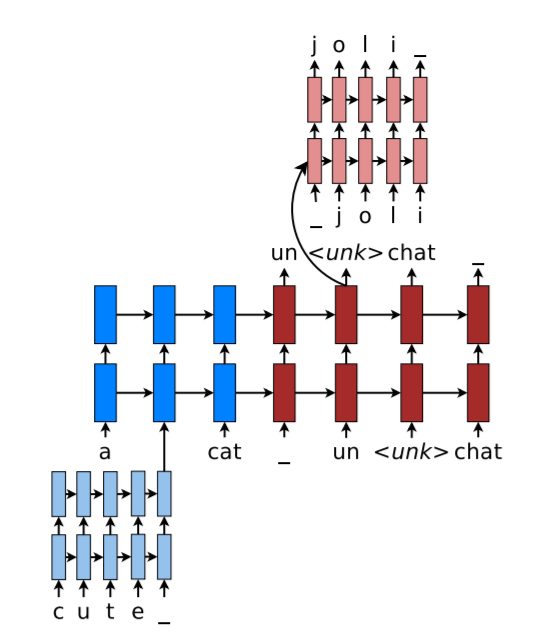
\includegraphics[width=0.5\textwidth]{images/char-decoder.PNG}
        \caption{A character-based decoder which is triggered if the word-based decoder produces an UNK. Figure courtesy of Luong \& Manning.}
        \label{fig:char-decoder}
    \end{center}
\end{figure}

We now describe the model in three sections:\\~\\
\textbf{Forward computation of Character Decoder}
Given a sequence of integers $x_1,\dots,x_n \in \Int$ representing a sequence of characters, we lookup their character embeddings $\bx_1,\dots,\bx_n \in \Real^{e_\text{char}}$ and pass these as input into the (unidirectional) LSTM, obtaining hidden states $\bh_1,\dots,\bh_n$ and cell states $\bc_1,\dots,\bc_n$:
\begin{equation}
    \bh_t, \bc_t = \text{CharDecoderLSTM}(\bx_t, \bh_{t-1}, \bc_{t-1}) \enspace \text{where} \enspace \bh_t, \bc_t \in \Real^h
\end{equation}
where $h$ is the hidden size of the CharDecoderLSTM.
The initial hidden and cell states $\bh_0$ and $\bc_0$ are both set to %\comment{Michael refine this to something more specific like `computed from the combined output vector using a two-layer feedforward net' or whatever}
the \textit{combined output vector} (refer to Assignment 4) for the current timestep of the main word-level NMT decoder.

For every timestep $t \in \{1,\dots,n\}$ we compute scores (also called logits) $\bs_t \in \Real^{V_\text{char}}$:
\begin{equation} \label{eq:decoder_logits}
    \bs_t = \bW_\text{dec} \bh_t + \bb_\text{dec} \in \mathbb{R}^{V_{char}}
\end{equation}
where the weight matrix $\bW_\text{dec} \in \mathbb{R}^{V_\text{char} \times h}$ and the bias vector $\bb_\text{dec} \in \mathbb{R}^{V_\text{char}}$.
If we passed $\bs_t$ through a softmax function, we would have the probability distribution for the next character in the sequence.
% The results of this computation are the sequence $(\bs_1, ..., \bs_n)$ and the final state $\bh_{n}$.

\textbf{Training of Character Decoder}
When we train the NMT system, we train the character decoder on \textit{every} word in the target sentence (not just the words represented by \texttt{<UNK>}).
For example, on a particular step of the main NMT decoder, if the target word is \texttt{music} then the input sequence for the CharDecoderLSTM is $[x_1,\dots,x_n] = [\texttt{<START>,m,u,s,i,c}]$ and the target sequence for the CharDecoderLSTM is $[x_2,\dots,x_{n+1}] = [\texttt{m,u,s,i,c,<END>}]$.

We pass the input sequence $x_1,\dots,x_n$, (along with the initial states $\bh_0$ and $\bc_0$ obtained from the combined output vector) into the CharDecoderLSTM, thus obtaining scores $\bs_1,\dots,\bs_n$ which we will compare to the target sequence $x_2,\dots,x_{n+1}$.
We optimize with respect to sum of the cross-entropy loss:
\begin{align}
    \bp_t &= \text{softmax}(\bs_t) \in \Real^{V_\text{char}} \qquad \forall t\in \{1,\dots,n\} \\
    \text{loss}_\text{char\_dec} &= - \sum_{t=1}^n \log \bp_t (x_{t+1}) \in \Real
\end{align}
Note that when we compute $\text{loss}_\text{char\_dec}$ for a batch of words, we take the sum (not average) across the entire batch.
On each training iteration, we add $\text{loss}_\text{char\_dec}$ to the loss of the word-based decoder, so that we simultaneously train the word-based model and character-based decoder.

\paragraph{Decoding from the Character Decoder}
At test time, first we produce a translation from our word-based NMT system in the usual way (e.g. a decoding algorithm like beam search).
If the translation contains any \texttt{<UNK>} tokens, then for each of those positions, we use the word-based decoder's combined output vector to initialize the CharDecoderLSTM's initial $\bh_0$ and $\bc_0$, then use CharDecoderLSTM to generate a sequence of characters.

To generate the sequence of characters, we use the \textit{greedy decoding} algorithm, which repeatedly chooses the most probable next character, until either the \texttt{<END>} token is produced or we reach a predetermined \texttt{max\_length}.
The algorithm is given below, for a single example (not batched).

\begin{algorithm}
\caption{Greedy Decoding}\label{alg:greedy}
\textbf{Input}: Initial states $\bh_0, \bc_0$ \\
\textbf{Output}: \texttt{output\_word} generated by the character decoder (doesn't contain \texttt{<START>} or \texttt{<END>})
\begin{algorithmic}[1]
    \Procedure{decode\_greedy}{}
    \State $\texttt{output\_word} \gets []$ 
    \State $\texttt{current\_char} \gets \texttt{<START>}$
    \For {$t = 0, 1, ..., \texttt{max\_length}-1$}
        \State    ${\bf h}_{t+1}, {\bf c}_{t+1} \gets \operatorname{CharDecoder}(\texttt{current\_char}, \bh_t, \bc_t)$ \Comment{use last predicted character as input}
        \State $\bs_{t+1} \gets \bW_\text{dec} \bh_{t+1} + \bb_\text{dec}$ \Comment{compute scores}
        \State $\bp_{t+1} \gets \text{softmax} (\bs_{t+1})$ \Comment{compute probabilities}
        \State $\texttt{current\_char} \gets \operatorname{argmax}_c\ \bp_{t+1}(c)$ \Comment{the most likely next character}
        \If {\texttt{current\_char}=\texttt{<END>}}
            \State \textbf{break}
        \EndIf
        \State $\texttt{output\_word} \gets \texttt{output\_word} + [\texttt{current\_char}]$ \Comment{append this character to output word}
    \EndFor
    \State \textbf{return} $\texttt{output\_word}$
    \EndProcedure
\end{algorithmic}
\end{algorithm}

\newpage

\subsection*{Implementation}
At the end of this section, you will train the full NMT system (with character-encoder and character-decoder). 
As in the previous assignment, we strongly advise that you first develop the code locally and ensure it does not crash, before attempting to train it on your VM.
Finally, \textbf{make sure that your VM is turned off whenever you are not using it.}
\begin{enumerate}[(a)]
    \item \points{2a} Write the \texttt{\_\_init\_\_} function for the \texttt{CharDecoder} module in \texttt{src/submission/char\_decoder.py}.
    
    \item \points{2b} Write the \texttt{forward()}  function in \texttt{src/submission/char\_decoder.py}. This function takes input $x_1,\dots,x_n$ and $(\bh_0, \bc_0)$ (as described in the \textbf{Forward computation of the character decoder} section) and returns $\bs_1,\dots,\bs_n$ and $(\bh_n, \bc_n)$.

    \item \points{2c} Write the \texttt{train\_forward()} function in \texttt{src/submission/char\_decoder.py}. This function computes $\text{loss}_\text{char\_dec}$ summed across the whole batch. Hint: Carefully read the documentation for \texttt{nn.CrossEntropyLoss}.

    \item \points{2d} Write the \texttt{decode\_greedy()} function in \texttt{src/submission/char\_decoder.py} to implement the algorithm \textsc{decode\_greedy}. 
    Note that although Algorithm \ref{alg:greedy} is described for a single example, your implementation must work over a batch.
    Algorithm \ref{alg:greedy} also indicates that you should break when you reach the \texttt{<END>} token, but in the batched case you might find it more convenient to complete all \texttt{max\_length} steps of the for-loop, then truncate the \texttt{output\_word}s afterwards.

    \item \points{2e} \label{qn:run_tiny_dec} (coding) Once you have thoroughly checked your implementation of the \texttt{CharDecoder} functions (checking much more than just the basic test sanity checks!), it's time to do the `small training run' check.
    
    Confirm that you're in the proper conda environment and then execute the following command on your \textbf{local} machine to check if your model overfits to a small subset of the training data.
\begin{lstlisting}
(XCS224N)$ sh run.sh train_local_q2
(XCS224N)$ sh run.sh test_local_q2
\end{lstlisting}

    Running these should take around 10 minutes (but this depends on your local machine). 
    You should observe the average loss go down to near 0 and average perplexity on train and dev set go to 1 during training. Once you run the test, you should observe BLEU score on the test set higher than 99.00. 
    If you don't observe these things, you probably need to go back to debug!
    
    \item \points{2f} \label{qn:final_train} Now that we've implemented both the character-based encoder and the character-based decoder, it's finally time to train the full system!

    Connect to your VM and activate the environment that you created for Assignment 4:
\begin{lstlisting}
$ conda activate XCS224N
(XCS224N)$
\end{lstlisting}

        Once your VM is configured and you are in a tmux session (refer to \href{https://docs.google.com/document/d/10J520Vnb1LnAMo0qgSYpG5cEEbomqQ371NIqg1IAv-4/edit?usp=sharing}{XCS224N Azure Guide} more information on tmux) execute:
        \begin{center}
            \texttt{sh run.sh train}
        \end{center}
    This should take between \textbf{8-12} hours to train on the VM, though time may vary depending on your implementation and whether or not the training procedure hits the early stopping criterion. 
    
    Run your model on the test set using:
        \begin{center}
            \texttt{sh run.sh test}
        \end{center}
    and \textbf{ensure that the output file \texttt{outputs/test\_outputs\_soln.txt} is present and unmodified -- this will be included in your submission, and we'll use it to evaluate the final BLEU score}
    
    Given your BLEU score $b$, here's how your points will be determined for this sub-problem: \newline \\
    \begin{tabular}{c c}
        BLEU Score & Points \\ \hline 
        $0 \le b < 10 $ & 0 \\ % 10 = number we added in A4
        $10 \le b < 16$ & 2 \\ % 
        $16 \le b$ & 6 \\ % 16 = should be doable on their local, 
        % 24.25 and above & 4 \\ % 24.2 = our solution
    \end{tabular}

\end{enumerate}
\clearpage

\textbf{Deliverables}

For this assignment, please submit all files within the |src/submission| subdirectory, as well as your q1, q2, and final test outputs, |outputs/test_outputs_soln.txt| (created on the VM).  This includes:
\begin{itemize}
    \item |src/submission/__init__.py|
    \item |src/submission/char_decoder.py|
    \item |src/submission/cnn.py|
    \item |src/submission/highway.py|
    \item |src/submission/model_embeddings.py|
    \item |src/submission/nmt_model.py|
    \item |src/submission/utils.py|
    \item |src/submission/vocab.py|
    \item |src/outputs/test_outputs_soln.py|
    \item |src/outputs/test_outputs_soln.py|
    \item |src/outputs/test_outputs_soln.py|
\end{itemize}   
